\ifx\doclanguage\english
\chapter{Design}

This chapter describes the layout of the thesis' proposed solution. The \ac{BDI} agents work in a \ac{MAS} via Jason AgentSpeak and communicate via solidity and python-based smart contracts. We would talk about the application's design objectives and general overview. We will also go through the application's design and functionality for both creating smart contracts independently and after doing so, as well as for creating agents. This chapter's prerequisites include understanding the design and architecture of blockchain, AgentSpeak, and \ac{AOP} as described in the previous chapter. The prior chapter's contents should be reviewed in order to fully comprehend the chapters that follow.

\section{Roadmap}
.......

\section{Model Description}

    \begin{figure}[h]
    \centering
      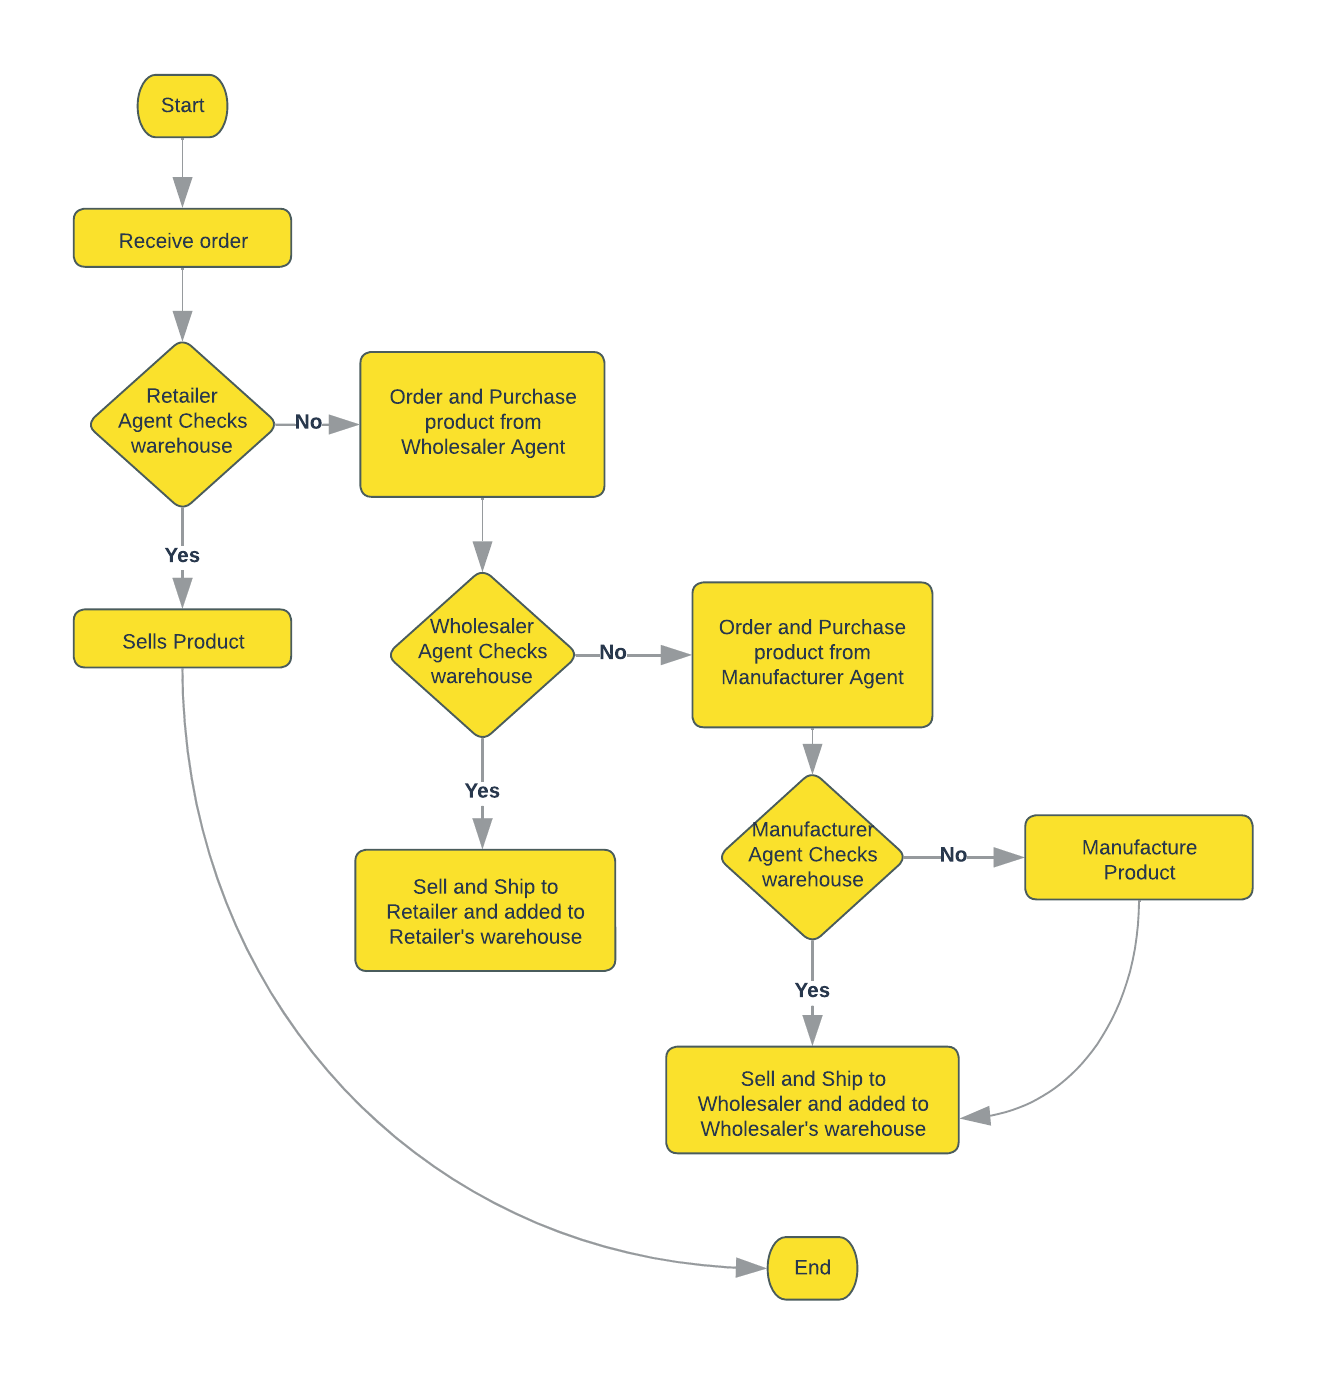
\includegraphics[width=10cm]{includes/figures/Flow Chart.png}
      \caption{Supply Chain Flow Chart}
      \label{Flow chart}
    \end{figure}


The application flow for the \textit{Smart contract development with Jason \ac{BDI} agents} is depicted in Figure  \ref{Flow chart}. These three agents, a manufacturer, a wholesaler, and a retailer, each perform a specific function in the supply chain. All three of the other agents are being invoked by another primary agent in the \ac{MAS}. Figure \ref{Sequence Diagram} may be used to demonstrate this.

   \begin{figure}[h]
    \centering
      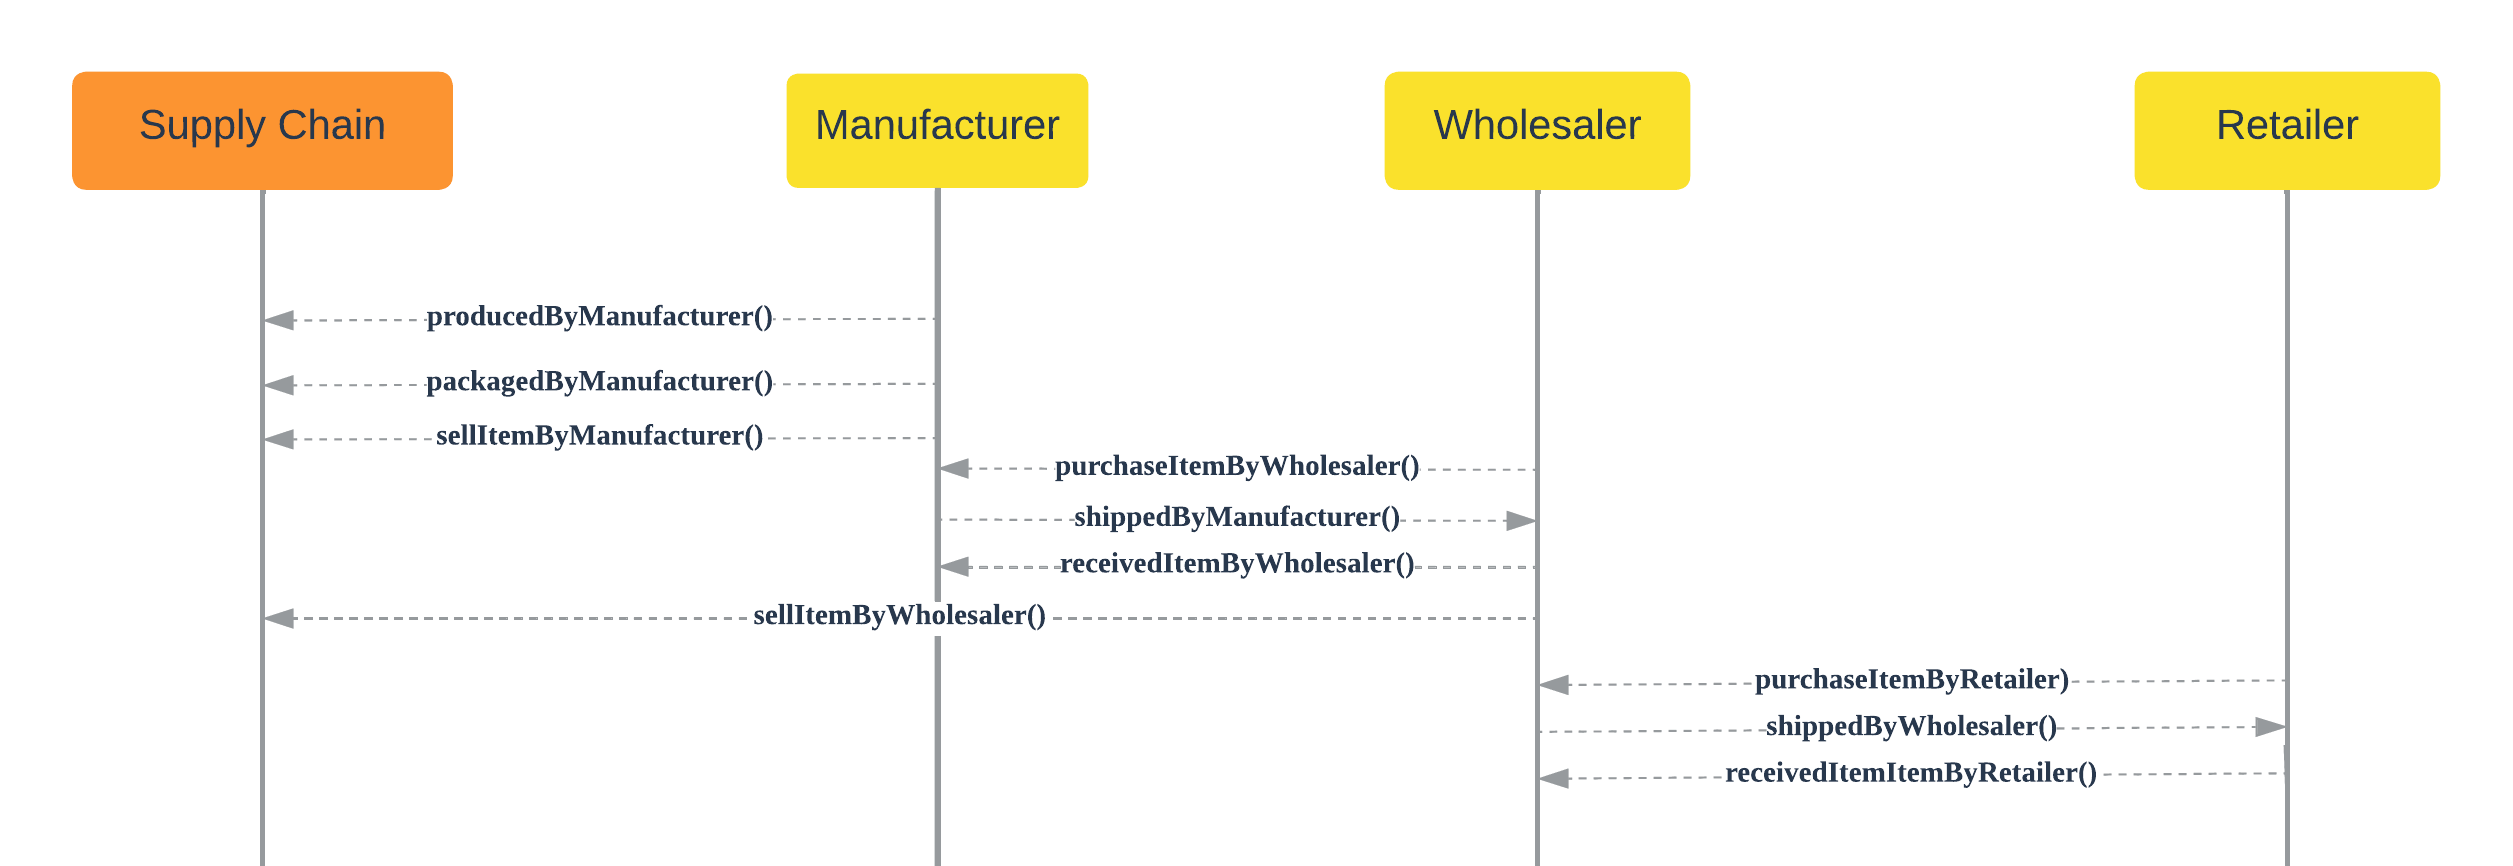
\includegraphics[width=\linewidth]{includes/figures/Sequence diagram.png} 
      \caption{Supply Chain Sequence Diagram}
      \label{Sequence Diagram}
    \end{figure}

\section{Design Goals}

\begin{itemize}

    \descitem{Autonomous}
    To fulfill the objectives assigned to an agent, autonomy simply implies being able to work autonomously. An autonomous agent, thus, at the very least, makes independent judgments about how to accomplish its given goals; these decisions (and subsequently, its actions) are within its own control and are not influenced by other forces.
    
    \descitem{Efficiency}
    Effectiveness strategies improve the functioning of a smart contract or lower the expenses connected with its use. These patterns can help operators and consumers save time and money.
    
    \descitem{Access Control Patterns}
    Particular smart contract functionalities are only accessible by certain people, according to access control rules. For a specific task, permissions and authorizations can be managed, such as limiting access to the admin. On a public blockchain ledger, where everyone can observe the contract but you want to limit who may do what within the contract, the ability to restrict access is especially helpful. Certain access control patterns, such multi-authorization, ownership, and role-based access control, have names that make it obvious what they are meant to do.
    
    \descitem{Goal-directed behaviour}
    If an agent has been assigned a specific objective, it is assumed that the agent would attempt to attain the goal. Proactivity eliminates completely passive actors who never strive to accomplish anything.

    \descitem{Reactiveness}
    Implementing an application that achieves an appropriate mix of goal-directed and reactive behavior becomes difficult. This is one of the primary design goals of AgentSpeak.
    
    \descitem {Security}
    Protection patterns are created to optimize a smart contract's level of security against any threat. Reentrancy attacks, overflow assaults, or the problematic behavior of the actual smart contracts are all prevented by using them. There are various different types of frequently utilized security patterns, which is not surprising given the quantity of assets connected to smart contracts. Numerous of these patterns, such as circuit breakers and evacuation plans, are intended to safeguard contracts against failure in the event that the worst occurs.
\end{itemize}

\section{Contracts Overview}   

While taking into consideration the scenario of a supply chain where all information on suppliers, recipients, products, and business circumstances is dispersed over supply chain databases.
It is possible to execute the sale of products or services as a transaction that is cryptographically signed by the seller and the buyer and attached to a smart contract for sales transactions. When the sale occurs and all other conditions, such as documentation and quality checks, are met, the execution of the transfer of the corresponding funds and rights can be enforced; in other words, smart contracts can ensure that collaborative and entrepreneurial processes are carried out correctly.

\vspace{.5cm}

As aforementioned, the terminology blockchain refers to two things: a distributed database and a data structure (i.e. a linked list of blocks containing transactions, where each block is cryptographically chained to the preceding one by incorporating their hash value and a cryptographic signature, in such a manner that changing an earlier block requires re-creating the whole chain since that block). The idea of smart contracts, which are scripts that run every time a specific kind of transaction takes place and may read and write to the blockchain, is related to the blockchain technology. Smart contracts enable parties to enforce the requirement that while one transaction occurs, other transactions also occur.

    \begin{figure}[h]
    \centering
      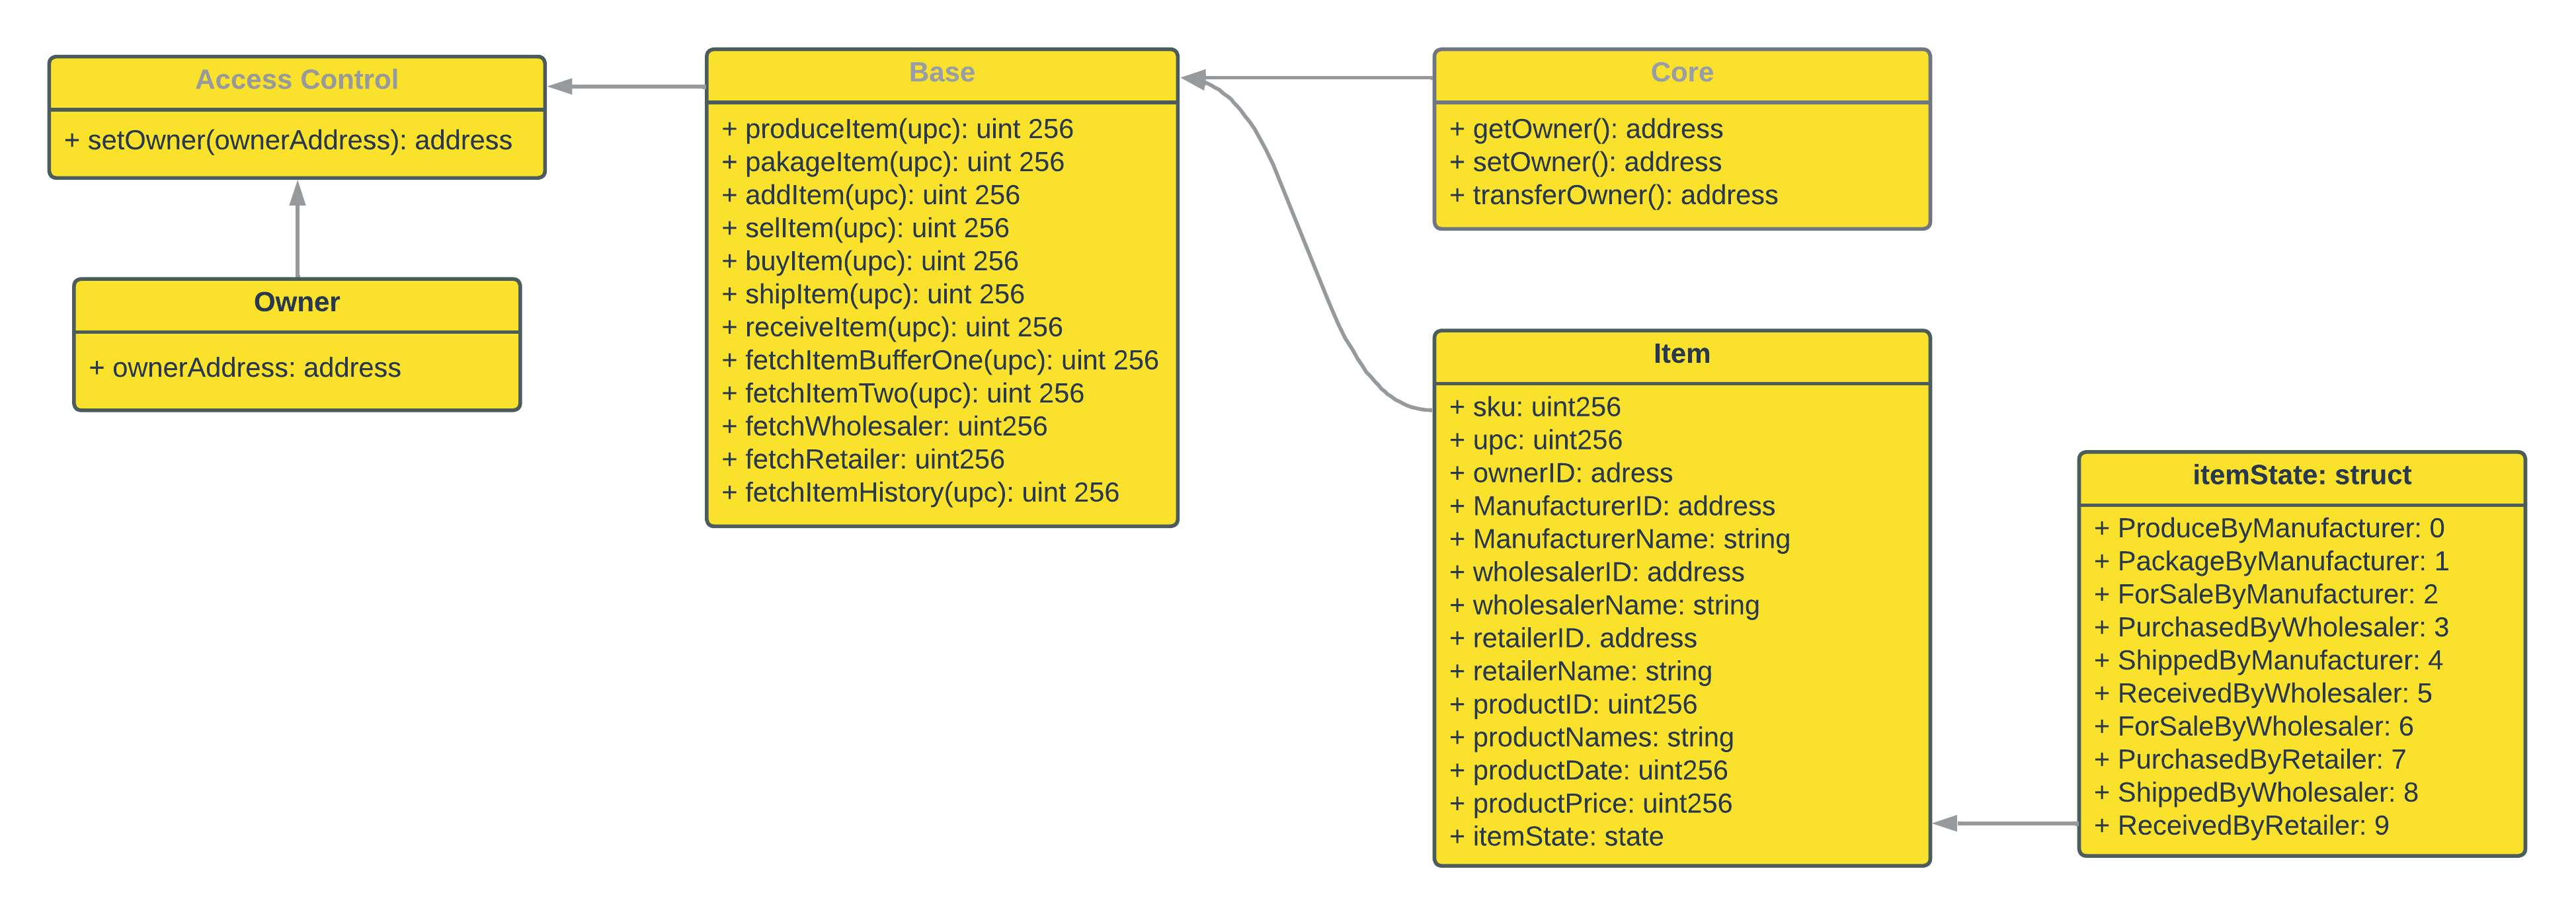
\includegraphics[width=15cm]{includes/figures/Data Model diagram.png} 
      \caption{Data Model Diagram}
      \label{Data Model diagram}
    \end{figure}
    
\vspace{.5cm}

The programming for smart contracts related supply chain is done using Solidity Language while keeping the version in mind in order to integrate it with the agent programming language so that they can work together. Smart contracts perform the following functions: (1) The product is produced by the manufacturer, (2) the manufacturer completes the packaging, (3) the product is placed on the market, (4) the wholesaler purchases the product, (5) the manufacturer ships the product, (6) the wholesaler receives the product, (7) the wholesaler places the product on the market, (8) the retailer purchases the product, (9) the wholesaler ships the product, and (10) the retailer receives the product as the final result.

\vspace{.5cm}

Each function is regarded as an event, and every event is given a state, as shown in Figure \ref{Data Model diagram}. It has always been a rule that each event must occur after the one before it has concluded. For example, a manufacturer cannot sell a product before producing it, while a wholesaler cannot receive a product before buying it. It is carried out with the aid of a state check. A product can also be tracked using the \ac{UPC} or by utilizing the \ac{SKU} to trace the entire batch.

\section{Agent Model}

An agent continually perceives its environment, makes decisions about how to act to achieve its objectives, and then takes action to alter the surroundings. The speech-act theory is commonly used to describe agent communication in \ac{MAS}. The speech-act hypothesis is based on the premise that language is action.

\vspace{.5cm}

\begin{figure}[h]
    \centering
      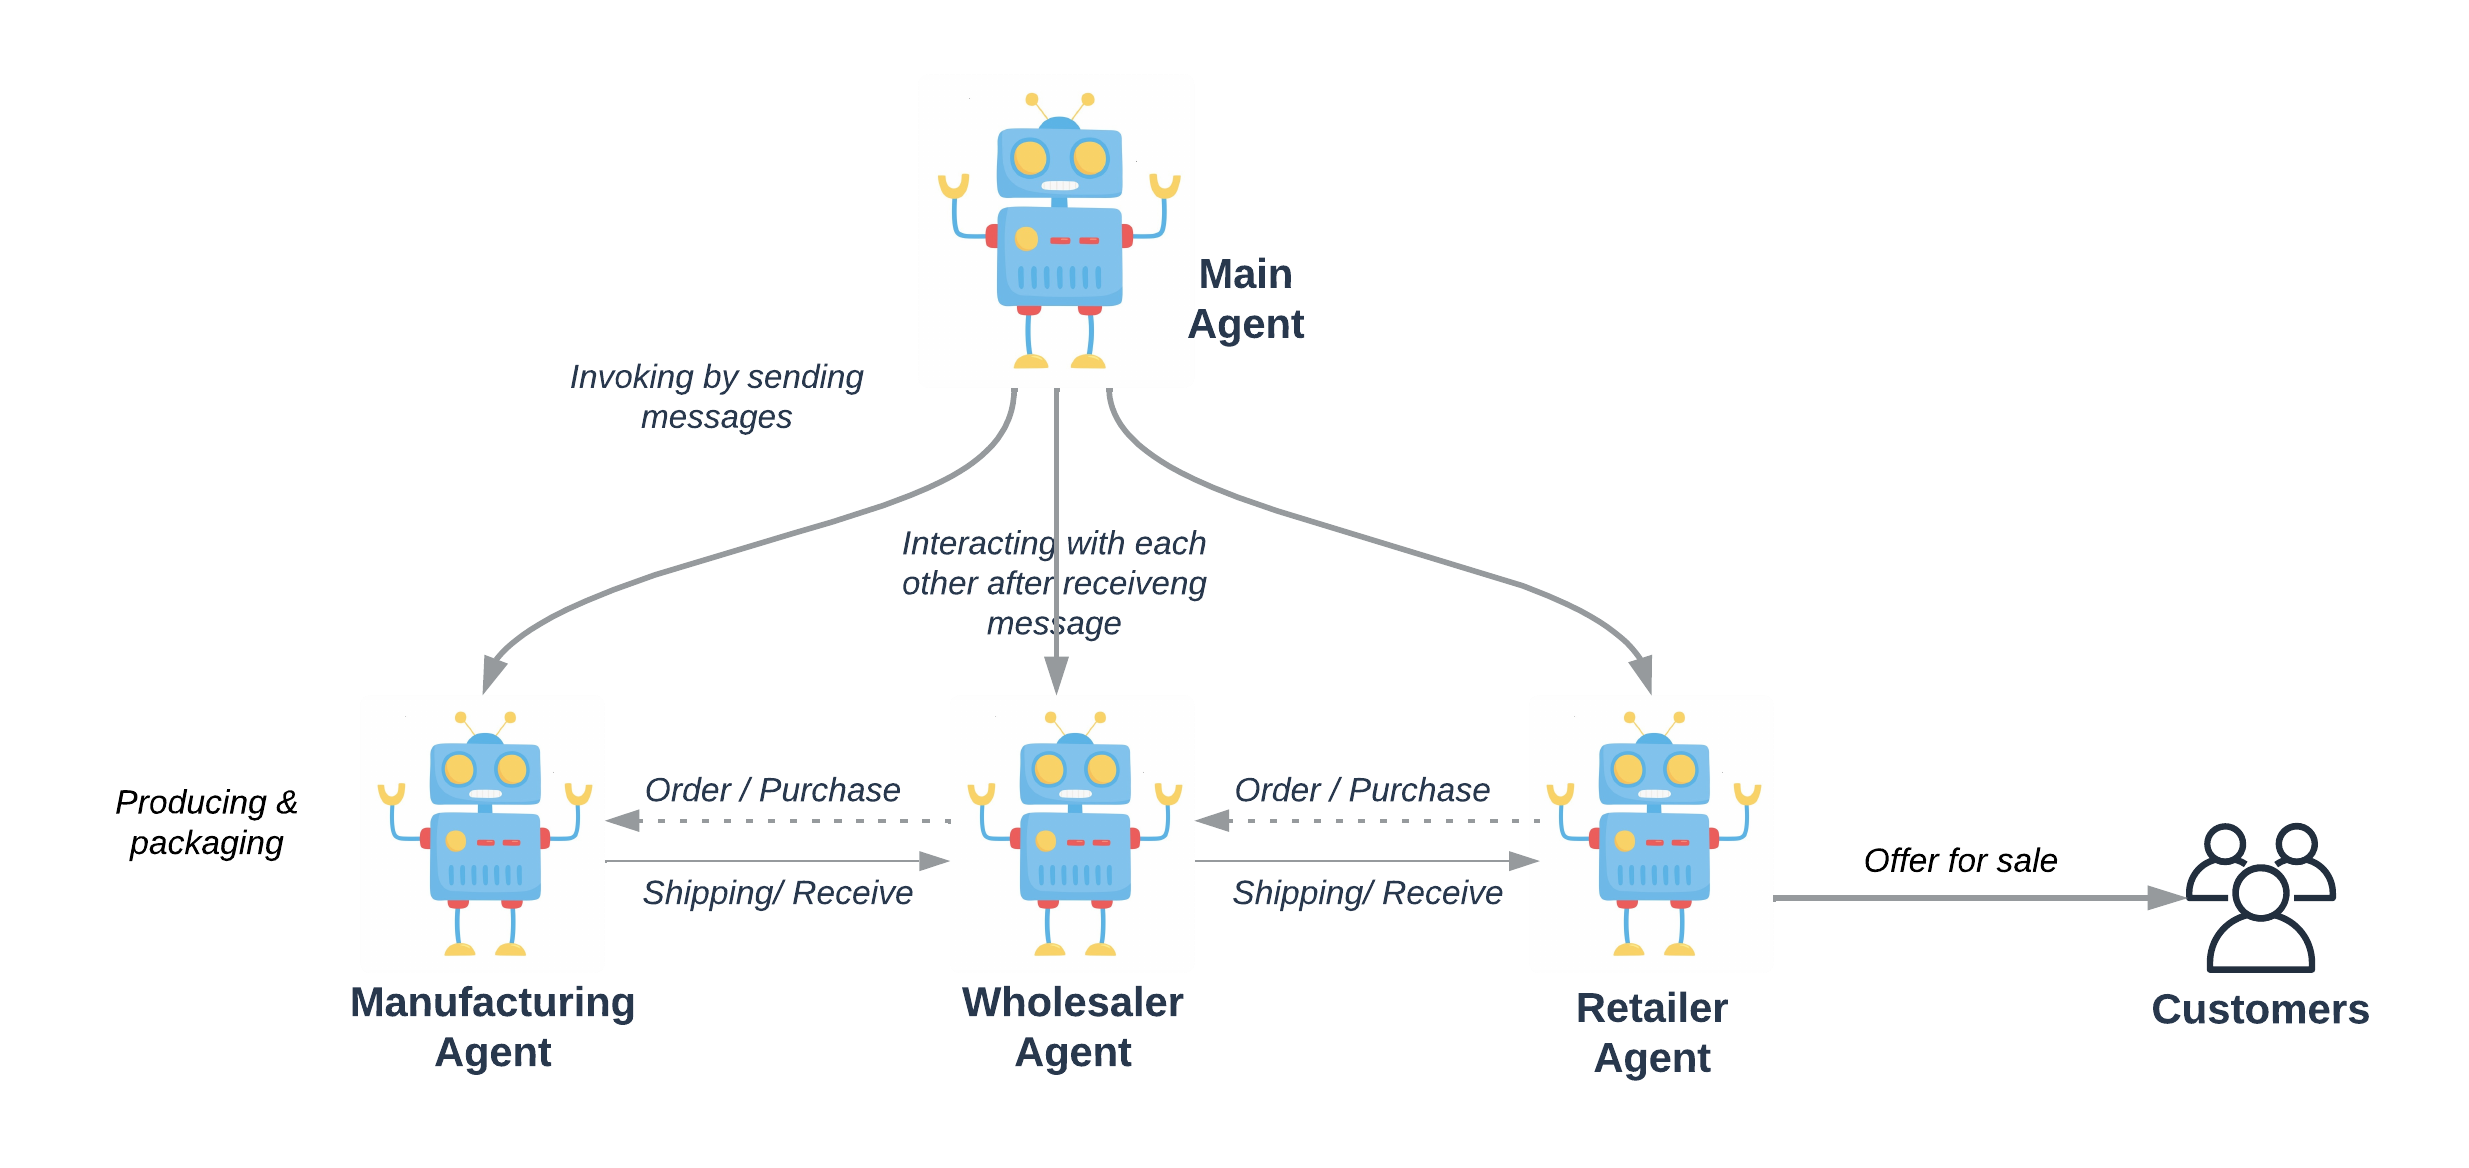
\includegraphics[width=\linewidth]{includes/figures/agent.png} 
      \caption{Agent Interaction in Supply chain}
      \label{Agent Interaction}
    \end{figure}
  

An agent program is run by the Jason interpreter. An agent uses a reasoning cycle to carry out its operations, which may be broken down into the following steps: first, it perceives the environment; second, it updates the belief base; third, it receives communication from other agents; fourth, it selects "socially acceptable" messages; fifth, it chooses an event; sixth, it retrieves all relevant plans; seventh, it determines the applicable plans; eighth, it chooses one applicable plan; and last, it executes one step of an intention.

\vspace{.5cm}

In our \ac{MAS}, each participant's function within the supply chain will be handled by an agent , see figure \ref{Agent Interaction}. The retailer agent will work to ensure that the product is available in the warehouse before ordering it from the wholesaler agent, who will then ask the wholesaler to check its inventory, get in touch with the manufacturer to produce the product, and ship it to the wholesaler, who will then send it to the retailer agent. There will be a \textit{main agent}, who will launch the retailer agent's efforts to sell items to consumers and also other agents by sending messages.